\documentclass[UTF8,12pt]{article}
\usepackage{ctex}
\usepackage{indentfirst}
\usepackage{color}
\usepackage{hyperref}
\usepackage{graphicx}
\usepackage{subfigure}
\usepackage{pdfpages}
\usepackage{listings}
\usepackage{afterpage}

\newcommand\myemptypage{
    \null
    \thispagestyle{empty}
    \addtocounter{page}{-1}
    \newpage
}

\hypersetup{
    hidelinks,
	colorlinks=true,
	allcolors=black,
	pdfstartview=Fit,
	breaklinks=true
}

\definecolor{dkgreen}{rgb}{0,0.6,0}
\definecolor{gray}{rgb}{0.5,0.5,0.5}
\definecolor{mauve}{rgb}{0.58,0,0.82}

\lstset{ %
  language=Octave,                % the language of the code
  basicstyle=\footnotesize,           % the size of the fonts that are used for the code
  numbers=left,                   % where to put the line-numbers
  numberstyle=\tiny\color{gray},  % the style that is used for the line-numbers
  stepnumber=2,                   % the step between two line-numbers. If it's 1, each line 
                                  % will be numbered
  numbersep=5pt,                  % how far the line-numbers are from the code
  backgroundcolor=\color{white},      % choose the background color. You must add \usepackage{color}
  showspaces=false,               % show spaces adding particular underscores
  showstringspaces=false,         % underline spaces within strings
  showtabs=false,                 % show tabs within strings adding particular underscores
  frame=single,                   % adds a frame around the code
  rulecolor=\color{black},        % if not set, the frame-color may be changed on line-breaks within not-black text (e.g. commens (green here))
  tabsize=2,                      % sets default tabsize to 2 spaces
  captionpos=b,                   % sets the caption-position to bottom
  breaklines=true,                % sets automatic line breaking
  breakatwhitespace=false,        % sets if automatic breaks should only happen at whitespace
  title=\lstname,                   % show the filename of files included with \lstinputlisting;
                                  % also try caption instead of title
  keywordstyle=\color{blue},          % keyword style
  commentstyle=\color{dkgreen},       % comment style
  stringstyle=\color{mauve},         % string literal style
  escapeinside={\%*}{*)},            % if you want to add LaTeX within your code
  morekeywords={*,...}               % if you want to add more keywords to the set
}


\setlength{\parindent}{2em}

\begin{document}

\begin{titlepage}
    \includepdf[pages={1}]{cover.pdf}
\end{titlepage}

\myemptypage

\begin{center}
    \tableofcontents
\end{center}
\newpage

\section{网络服务器搭建}
\subsection{采用技术}
\subsubsection{Tomcat}

Tomcat服务器是一个免费的开放源代码的Web 应用服务器,属于轻量级应用服务器,在中小型系统和并发访问用户不是很多的场合下被普遍使用,是开发和调试JSP程序的首选。

实际上Tomcat是Apache服务器的扩展,但运行时它是独立运行的,所以当你运行tomcat时,它实际上作为一个与Apache独立的进程单独运行的。

\subsubsection{Java Servlet}
Java Servlet是运行在Web服务器或应用服务器上的程序,它是作为来自Web浏览器或其他HTTP客户端的请求和 HTTP 服务器上的数据库或应用程序之间的中间层。

使用 Servlet,可以收集来自网页表单的用户输入,呈现来自数据库或者其他源的记录,还可以动态创建网页。

\subsection{生产环境}
\begin{itemize}
    \item 操作系统:Windows 11
    \item IDE:IntelliJ IDEA 2023.1.4
    \item 服务器:Tomcat 9.0.55
    \item Java版本:JDK 17.0.4.1
\end{itemize}

\subsection{Tomcat搭建过程}
\subsubsection{下载Tomcat}
Tomcat是开源的,直接在官网上下载就可以了

这里需要的是v9.0.55,因此在archives里面寻找,直接给出v9.0.55的下载地址,然后解压在目标地址就可以了,.zip免安装,解压并配置环境变量即可使用

\subsubsection{配置环境变量}
\begin{itemize}
    \item 新建CATALINA\_HOME,值为Tomcat的文件夹地址
    \item 建立Path,添加\%CATALINA\_HOME\%/lib,\%CATALINA\_HOME\%
    /bin,\%CATALINA\_HOME\%/lib/servlet-api.jar
\end{itemize}

\subsection{测试Tomcat}
\subsubsection{启动Tomcat方法一}
在'./apache-tomcat-9.0.55/bin'目录下,双击startup.bat即可启动Tomcat,双击shutdown.bat即可关闭Tomcat

在启动界面会出现中文乱码的界面,如下:
\begin{figure}[htbp]
    \centering
    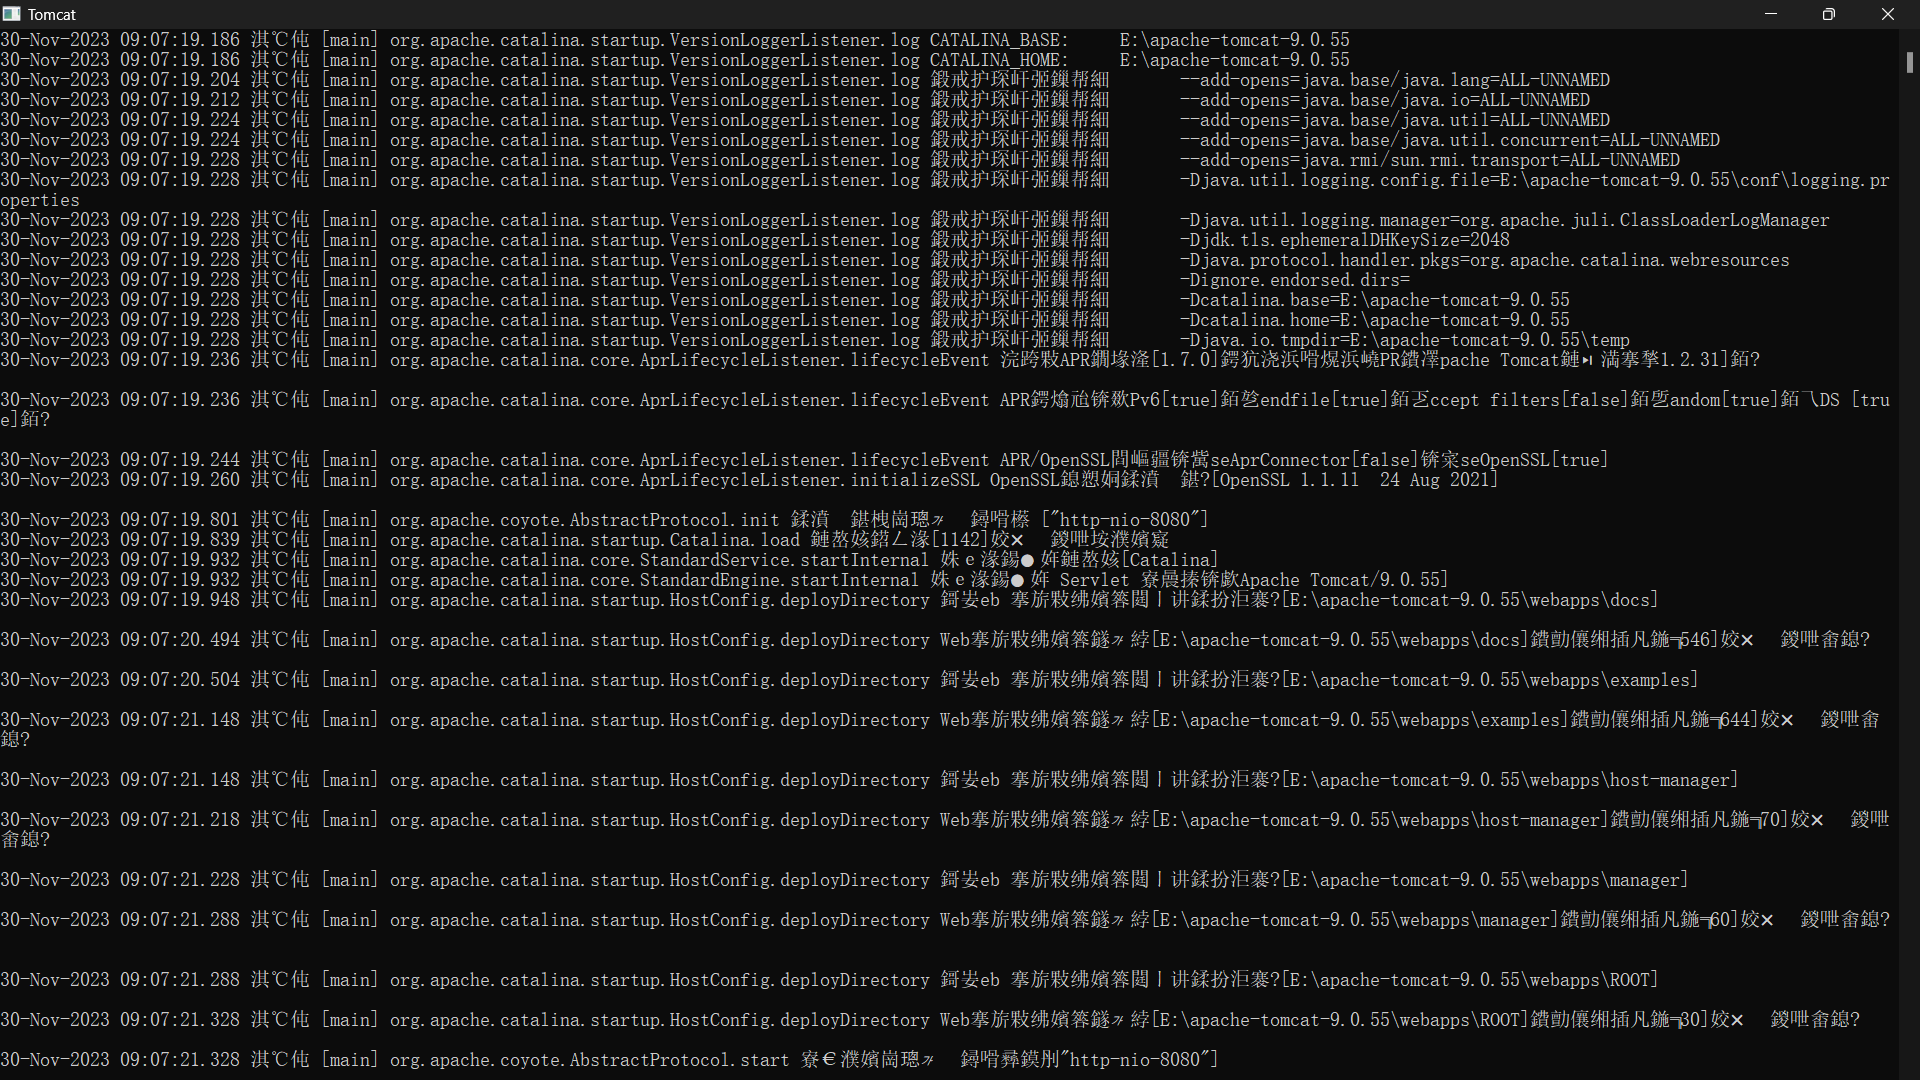
\includegraphics[width=0.6\textwidth]{imgs/1.png}
    \caption{Tomcat启动界面}
\end{figure}

解决方案是在'./apache-tomcat-9.0.55/conf/logging.properties'中,将

\begin{lstlisting}
    java.util.logging.ConsoleHandler.encoding = UTF-8
\end{lstlisting}

替换成

\begin{lstlisting}
    java.util.logging.ConsoleHandler.encoding = GBK
\end{lstlisting}

解决结果如下

\begin{figure}[htbp]
    \centering
    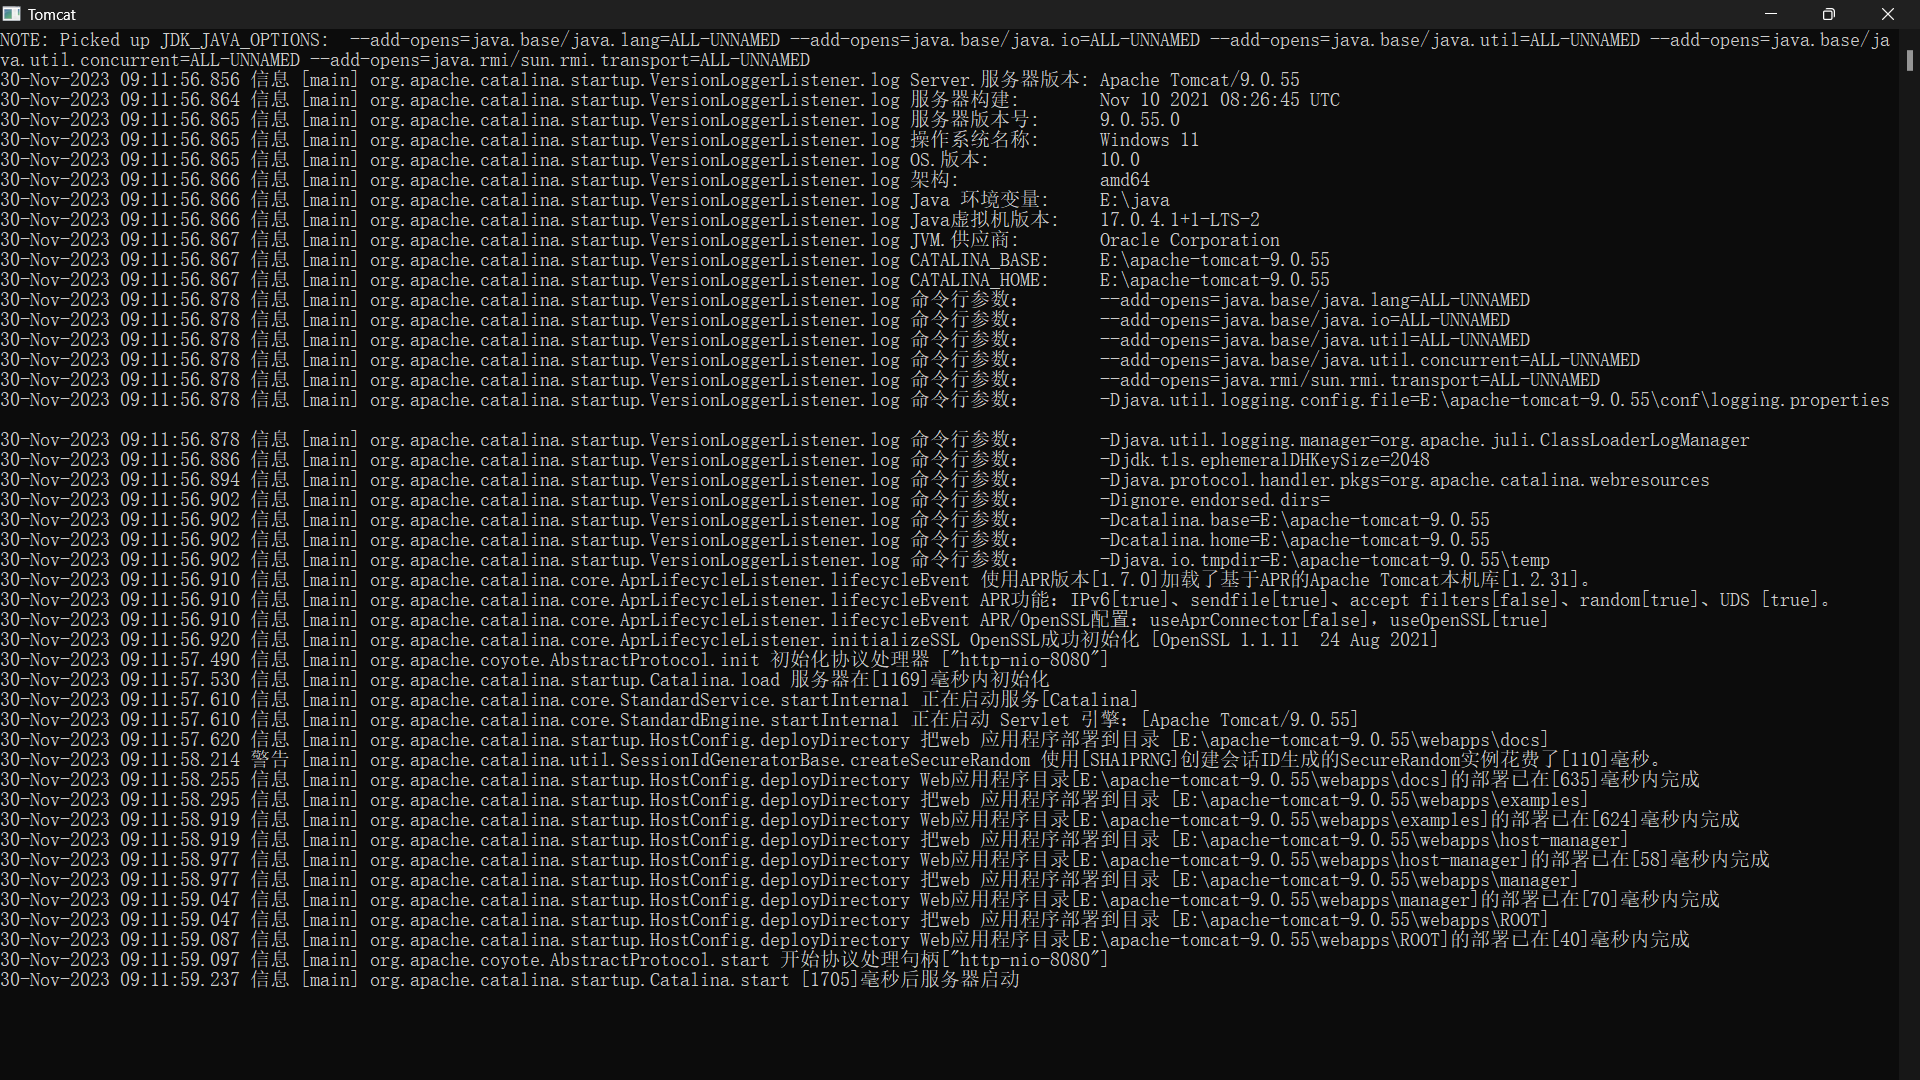
\includegraphics[width=0.6\textwidth]{imgs/2.png}
    \caption{Tomcat启动界面}
\end{figure}

\subsubsection{启动Tomcat方法二}
通过命令行打开Tomcat,进入'./apache-tomcat-9.0.55/bin'目录下,打开cmd,输入startup即可启动Tomcat

命令行出现:
\begin{lstlisting}[frame=shadowbox]
    Using CATALINA_BASE:   "E:\apache-tomcat-9.0.55"
    Using CATALINA_HOME:   "E:\apache-tomcat-9.0.55"
    Using CATALINA_TMPDIR: "E:\apache-tomcat-9.0.55\temp"
    Using JRE_HOME:        "E:\java"
    Using CLASSPATH:       "E:\apache-tomcat-9.0.55\bin\bootstrap.jar;E:\apache-tomcat-9.0.55\bin\tomcat-juli.jar"
    Using CATALINA_OPTS:   ""
\end{lstlisting}

并弹出Tomcat启动界面(如上),表明启动成功

输入shutdown即可关闭Tomcat

\subsubsection{访问Tomcat}
在启动Tomcat后,打开浏览器,输入地址'http://localhost:8080',弹出Tomcat自带的JSP界面,说明JDK和Tomcat搭建成功

\begin{figure}[htbp]
    \centering
    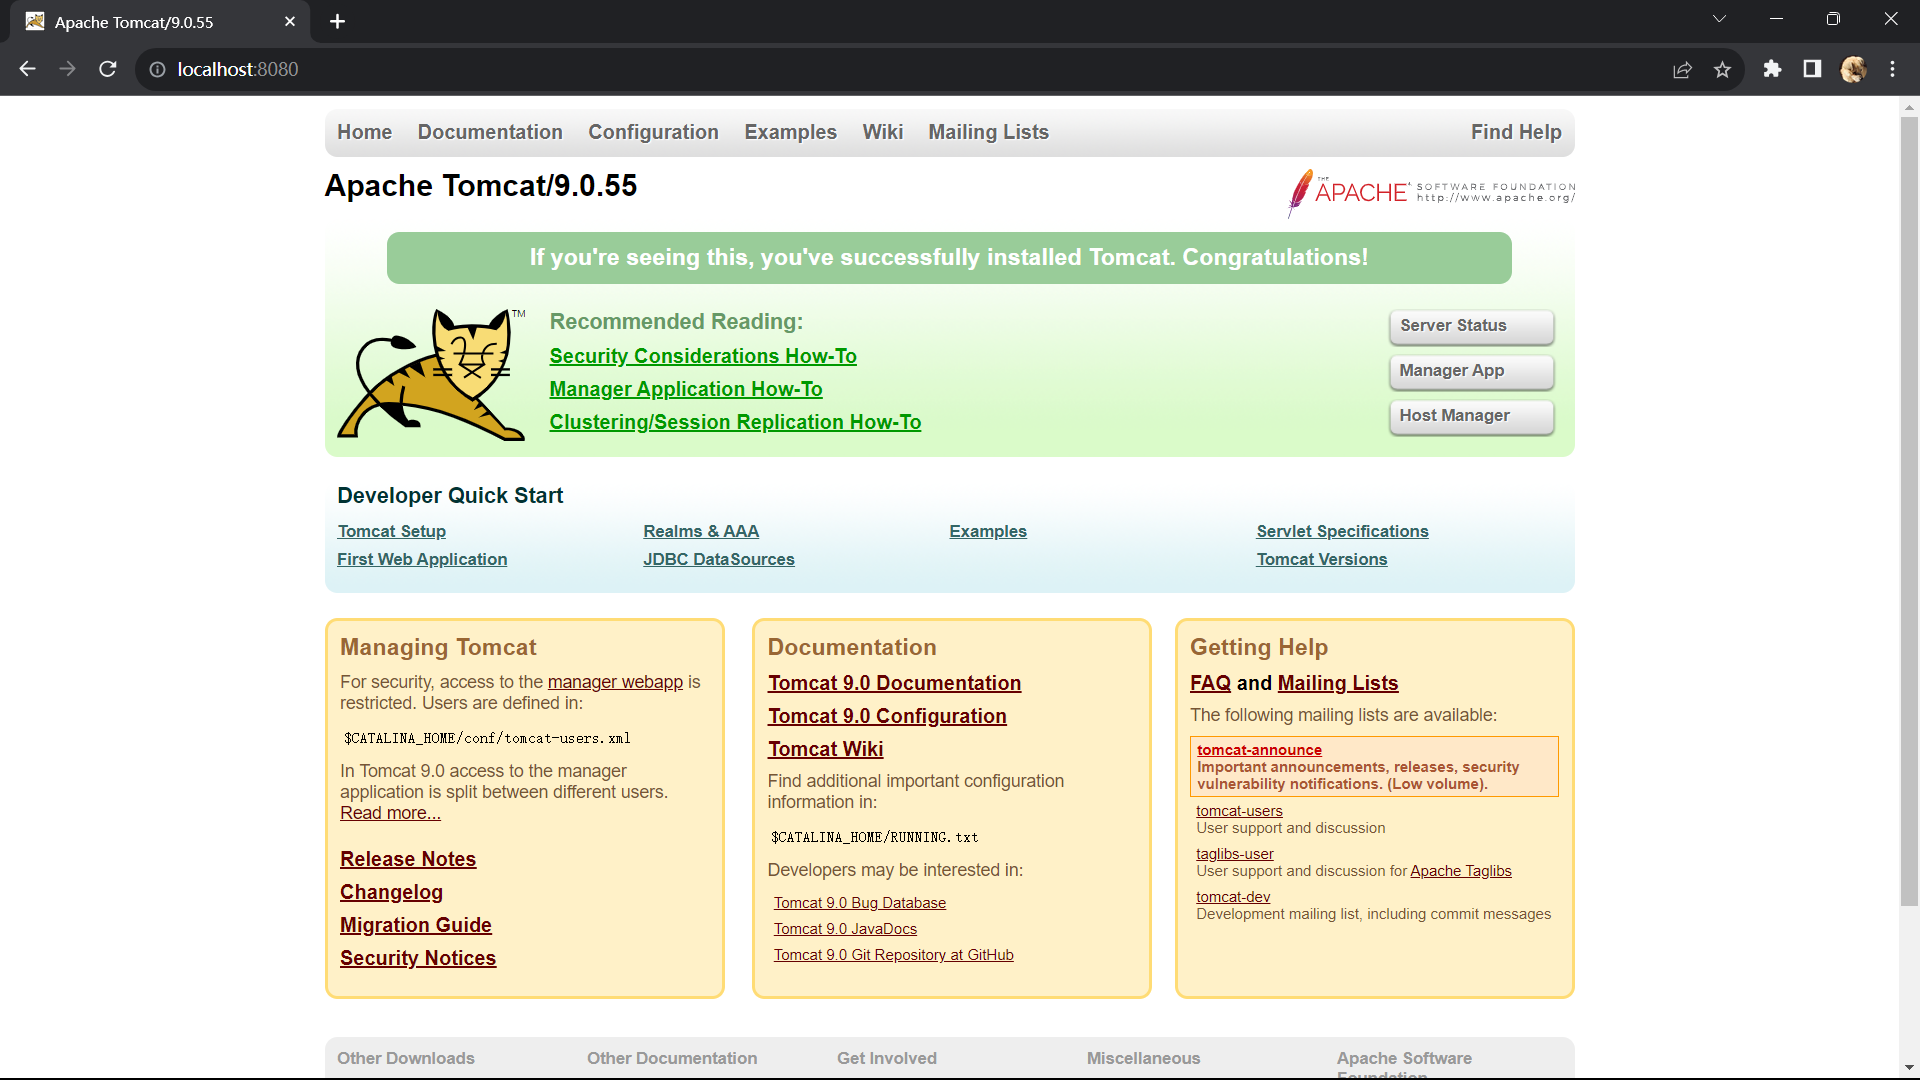
\includegraphics[width=1.0\textwidth]{imgs/3.png}
    \caption{Tomcat启动界面}
\end{figure}

\newpage

\section{数据库搭建}
\subsection{采用技术}
\subsubsection{MySQL}
MySQL是一种关系型数据库管理系统,关系数据库将数据保存在不同的表中,而不是将所有数据放在一个大仓库内,这样就增加了速度并提高了灵活性。

MySQL所使用的SQL语言是用于访问数据库的最常用标准化语言。

\subsubsection{JDBC}
JDBC是一种用于执行SQL语句的Java API,可以为多种关系数据库提供统一访问,它由一组用Java语言编写的类和接口组成。

JDBC提供了一种基准,据此可以构建更高级的工具和接口,使数据库开发人员能够编写数据库应用程序,同时,JDBC也是个商标名。

\subsection{生产环境}
\begin{itemize}
    \item 操作系统:Windows 11
    \item IDE:IntelliJ IDEA 2023.1.4
    \item DBMS:Navicat Premium 16.0.11
    \item 数据库:MySQL 5.7.31
    \item Java版本:JDK 17.0.4.1
\end{itemize}

\subsection{数据库设计}
\subsubsection{建立数据库}
在Navicat中新建数据库,命名为'hospital'
\begin{figure}[htbp]
    \centering
    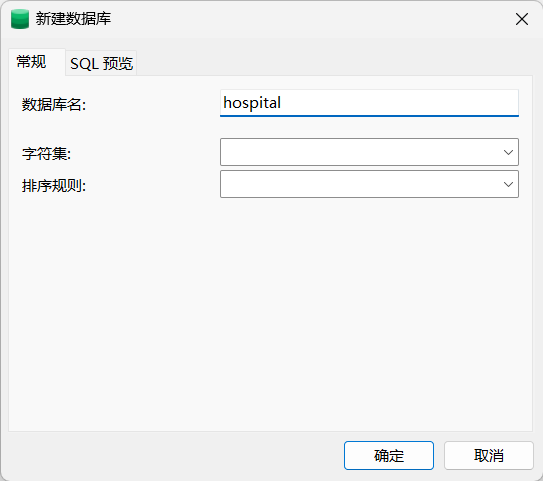
\includegraphics[width=0.6\textwidth]{imgs/4.png}
    \caption{新建数据库}    
\end{figure}

数据库的结构如下

\begin{lstlisting}[frame=shadowbox]
+--------------------+
| Tables_in_hospital |
+--------------------+
| depart             |
| doctor             |
| myorder            |
| schedule           |
| user               |
+--------------------+
\end{lstlisting}


\subsubsection{user表}
user表的主要字段有uid,uname,upsw,分别代表用户id,用户名,密码

\newpage

\begin{figure}[htbp]
    \centering
    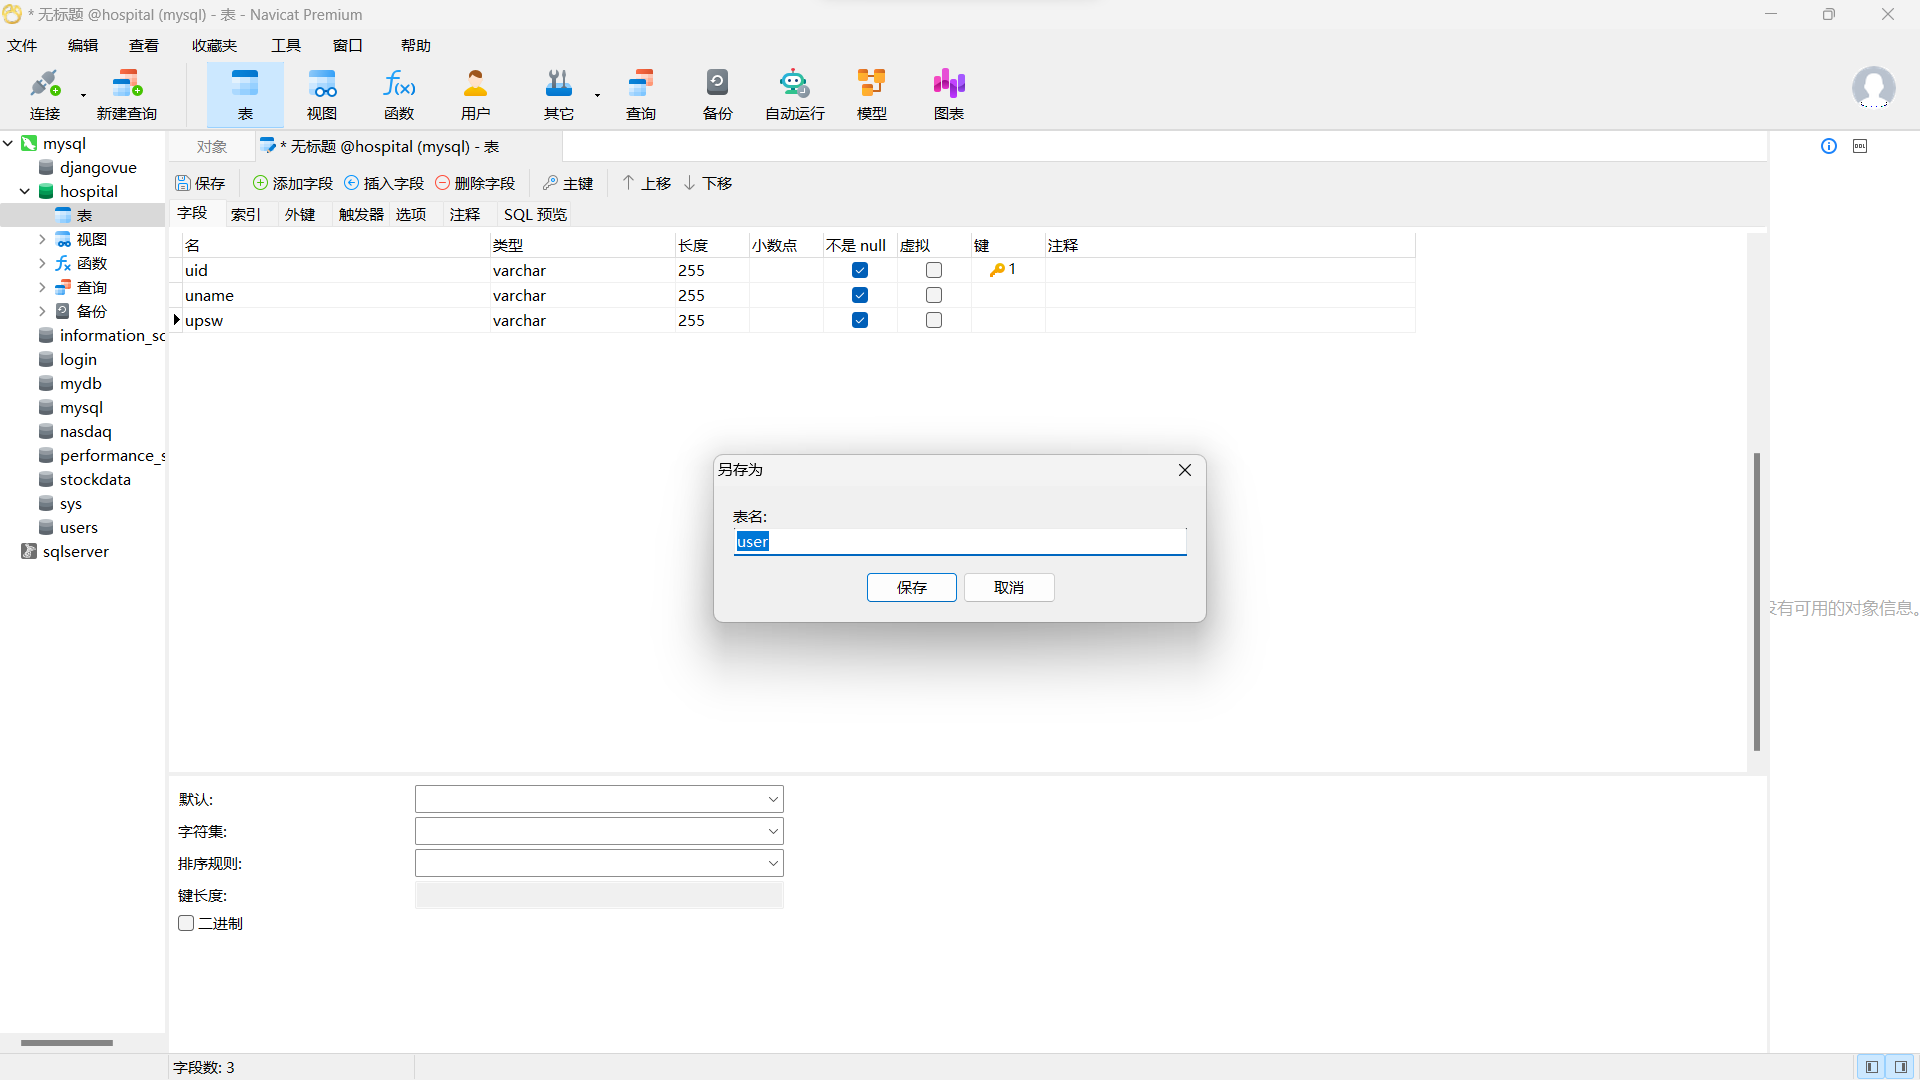
\includegraphics[width=0.6\textwidth]{imgs/5.png}
    \caption{user表}
\end{figure}

设计出的table结构如下

\begin{lstlisting}[frame=shadowbox]
+-------+--------------+------+-----+---------+-------+
| Field | Type         | Null | Key | Default | Extra |
+-------+--------------+------+-----+---------+-------+
| uid   | varchar(255) | NO   | PRI | NULL    |       |
| uname | varchar(255) | NO   |     | NULL    |       |
| upsw  | varchar(255) | NO   |     | NULL    |       |
+-------+--------------+------+-----+---------+-------+
\end{lstlisting}

\subsubsection{doctor表}

doctor表的主要字段有did,dname,dlevel,dinfo,departid,sex,ddetail分别代表医生id,医生姓名,医生职级,医生简介,医生所属科室id,医生性别,医生详细信息

\newpage

\begin{figure}[htbp]
    \centering
    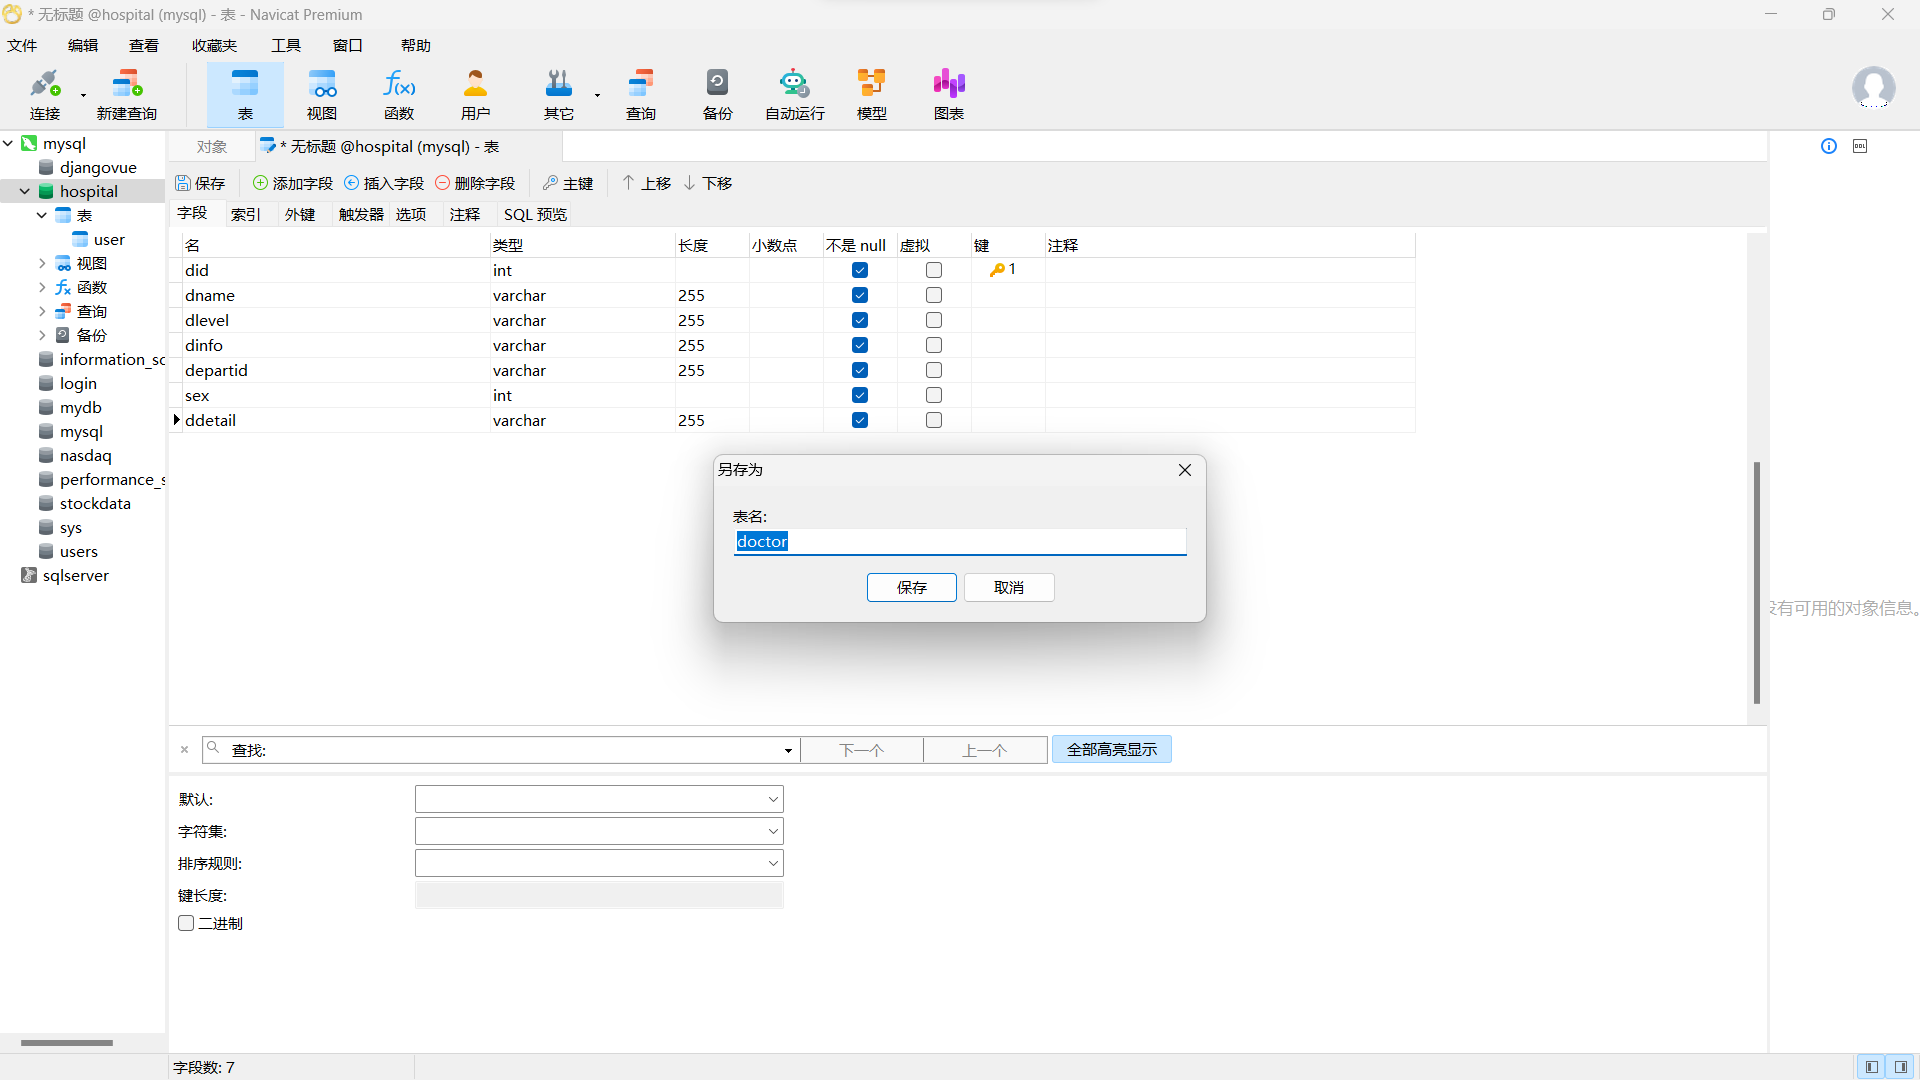
\includegraphics[width=0.9\textwidth]{imgs/6.png}
    \caption{doctor表}
\end{figure}

设计出的table结构如下

\begin{lstlisting}[frame=shadowbox]
+----------+--------------+------+-----+---------+-------+
| Field    | Type         | Null | Key | Default | Extra |
+----------+--------------+------+-----+---------+-------+
| did      | int(11)      | NO   | PRI | NULL    |       |
| dname    | varchar(255) | NO   |     | NULL    |       |
| dlevel   | varchar(255) | NO   |     | NULL    |       |
| dinfo    | varchar(255) | NO   |     | NULL    |       |
| departid | varchar(255) | NO   |     | NULL    |       |
| sex      | int(11)      | NO   |     | NULL    |       |
| ddetail  | varchar(255) | NO   |     | NULL    |       |
+----------+--------------+------+-----+---------+-------+
\end{lstlisting}

\subsubsection{depart表}

depart表的主要字段有departid,departname,分别代表科室id,科室名称

\begin{figure}[htbp]
    \centering
    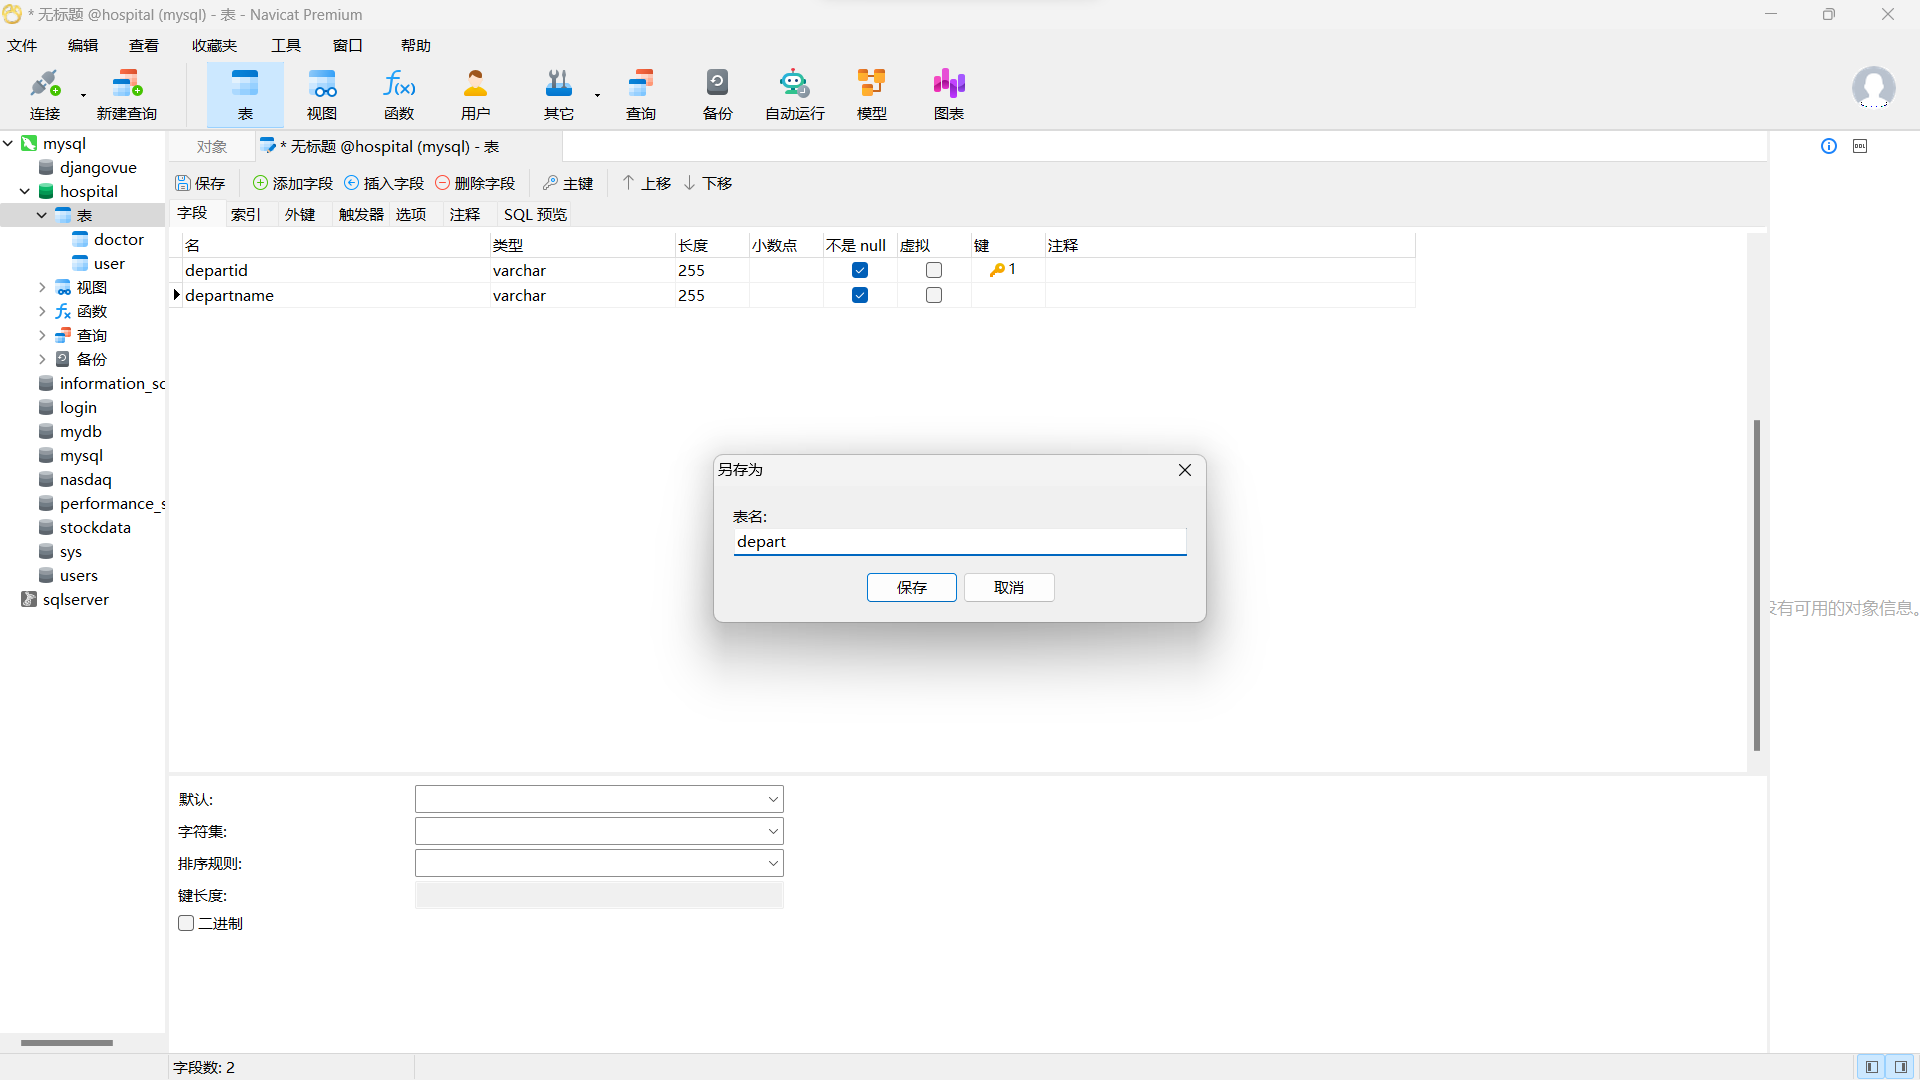
\includegraphics[width=0.8\textwidth]{imgs/7.png}
    \caption{depart表}
\end{figure}

设计出的table结构如下

\begin{lstlisting}[frame=shadowbox]
+------------+--------------+------+-----+---------+-------+
| Field      | Type         | Null | Key | Default | Extra |
+------------+--------------+------+-----+---------+-------+
| departid   | varchar(255) | NO   | PRI | NULL    |       |
| departname | varchar(255) | NO   |     | NULL    |       |
+------------+--------------+------+-----+---------+-------+
\end{lstlisting}

\subsubsection{schedule表}

schedule表的主要字段有sid,did,time,price分别代表排班id,医生id,排班时间,挂号费

\newpage

\begin{figure}[htbp]
    \centering
    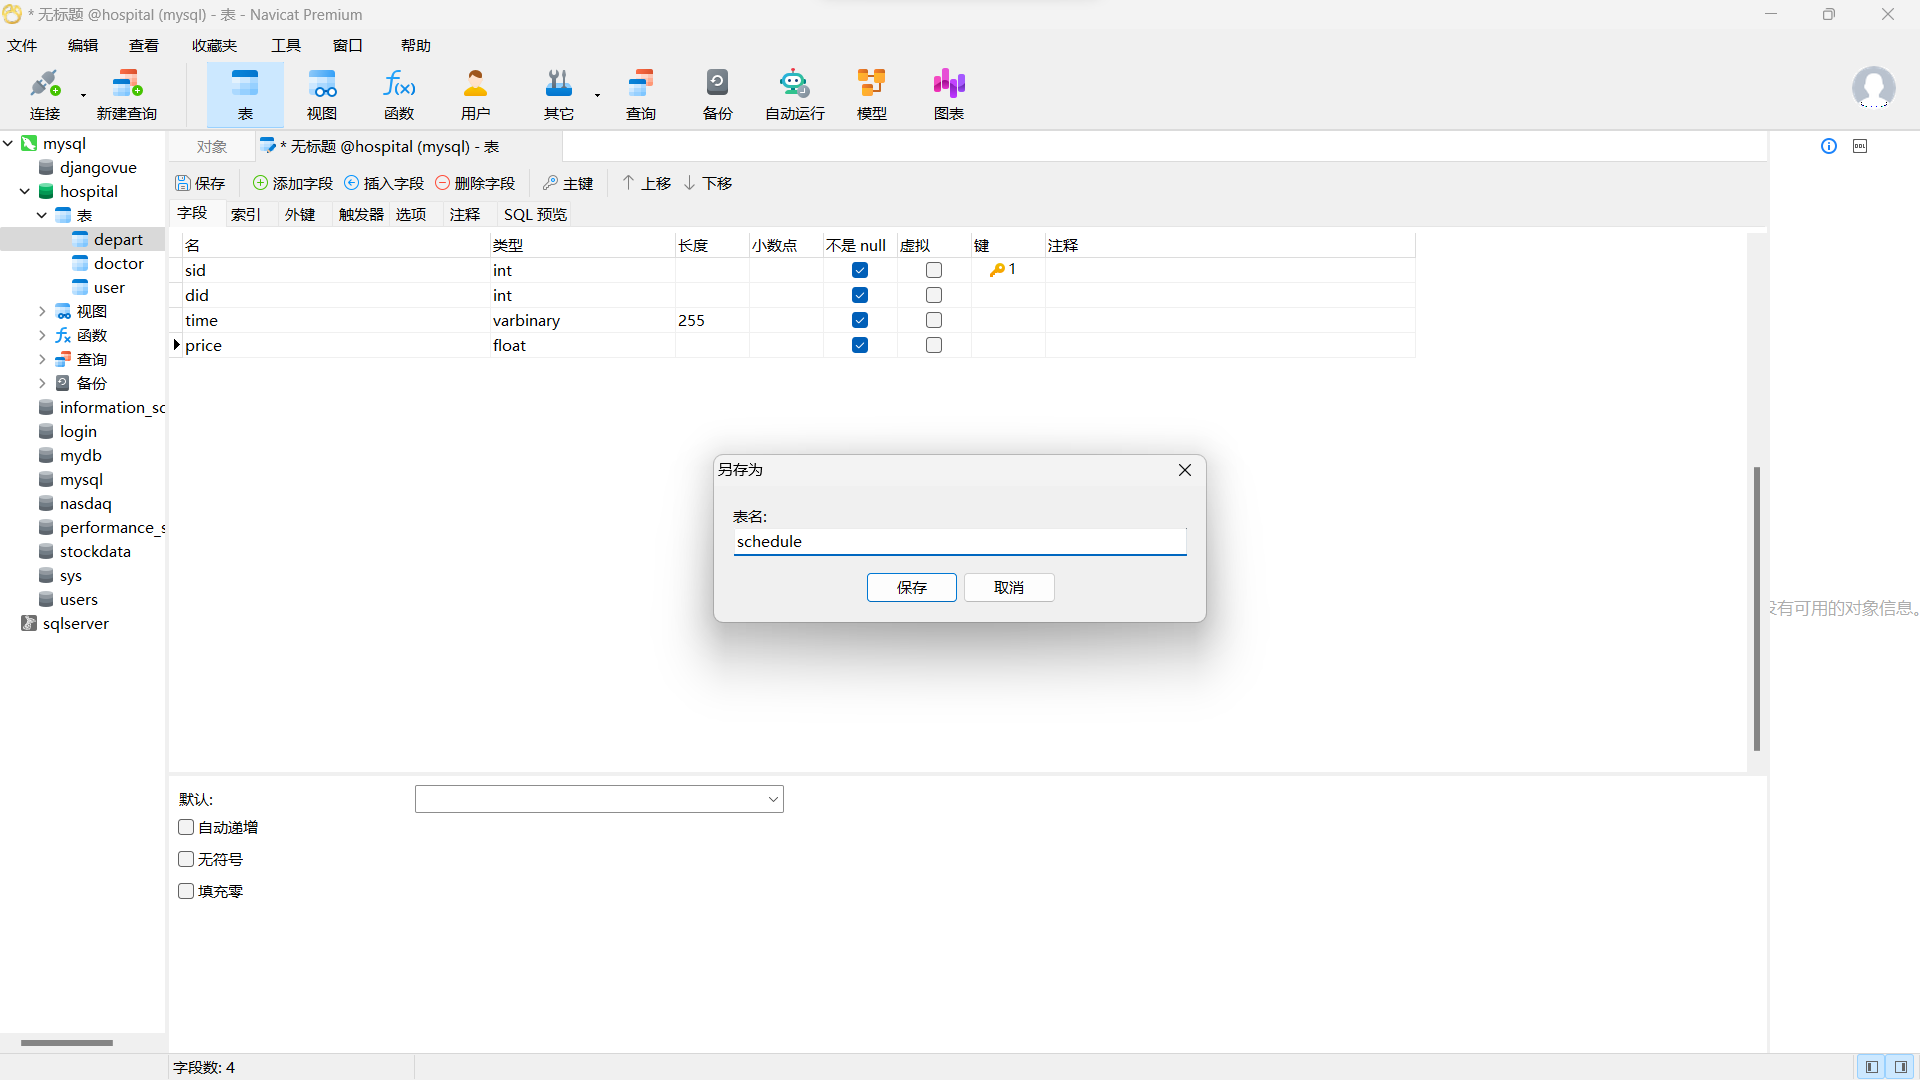
\includegraphics[width=0.8\textwidth]{imgs/8.png}
    \caption{schedule表}
\end{figure}

设计出的table结构如下

\begin{lstlisting}[frame=shadowbox]
+-------+----------------+------+-----+---------+-------+
| Field | Type           | Null | Key | Default | Extra |
+-------+----------------+------+-----+---------+-------+
| sid   | int(11)        | NO   | PRI | NULL    |       |
| did   | int(11)        | NO   |     | NULL    |       |
| time  | varbinary(255) | NO   |     | NULL    |       |
| price | float          | NO   |     | NULL    |       |
+-------+----------------+------+-----+---------+-------+
\end{lstlisting}

\subsubsection{myorder表}

myorder表的主要字段有oid,sid,did,分别代表订单id,排班id,医生id

\newpage

\begin{figure}[htbp]
    \centering
    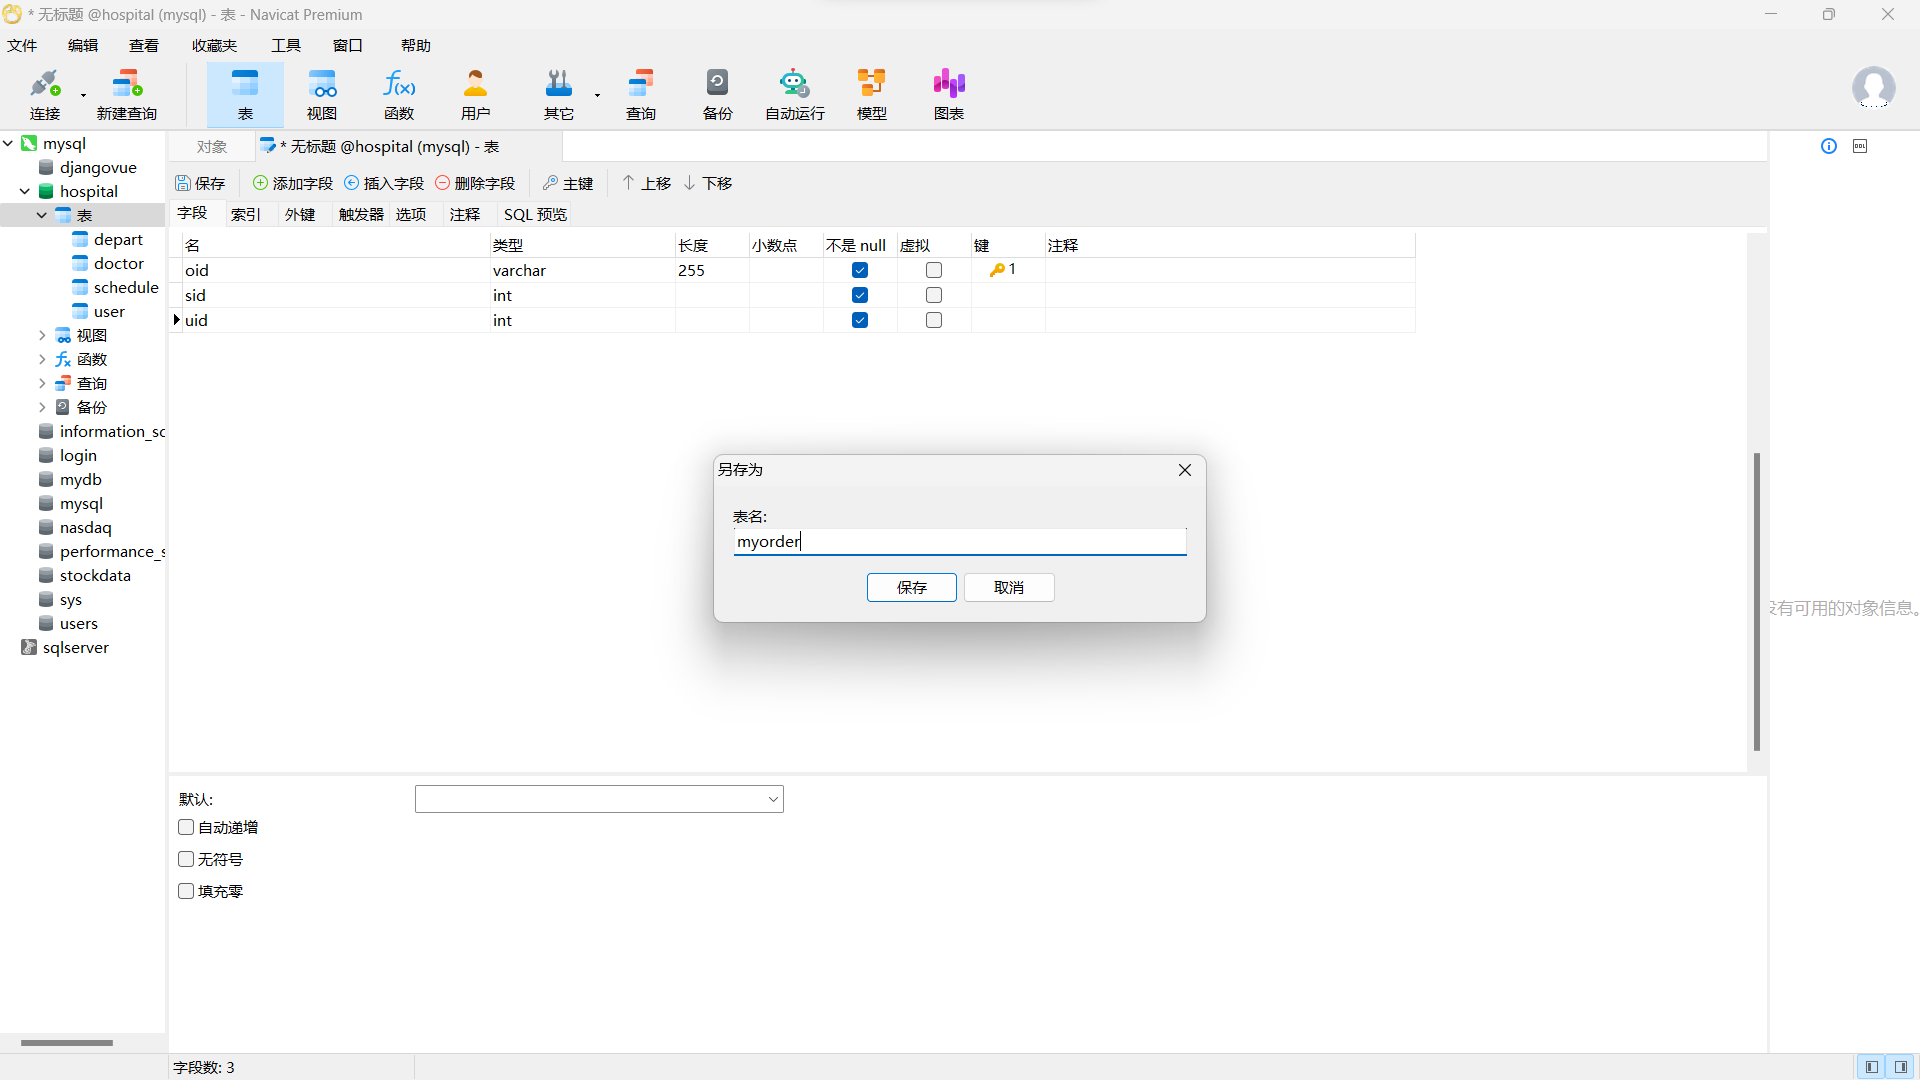
\includegraphics[width=0.8\textwidth]{imgs/9.png}
    \caption{myorder表}
\end{figure}

设计出的table结构如下

\begin{lstlisting}[frame=shadowbox]
+-------+--------------+------+-----+---------+-------+
| Field | Type         | Null | Key | Default | Extra |
+-------+--------------+------+-----+---------+-------+
| oid   | varchar(255) | NO   | PRI | NULL    |       |
| sid   | int(11)      | NO   |     | NULL    |       |
| uid   | int(11)      | NO   |     | NULL    |       |
+-------+--------------+------+-----+---------+-------+
\end{lstlisting}

\end{document}